% ISPA submission manuscript.
% Training-study measurements and constructed controller tests have distinct scopes.
\documentclass[conference,compsoc]{IEEEtran}

\usepackage[T1]{fontenc}
\usepackage{amsmath,amssymb}
\interdisplaylinepenalty=2500
\usepackage{booktabs,multirow,array}
\usepackage{threeparttable}
\usepackage{graphicx}
\usepackage{xcolor}
\usepackage{flafter} % Keep floats after their source position and first mention.
\usepackage{placeins} % Keep experimental floats out of the conclusion and references.
\usepackage[nocompress]{cite}
\usepackage{xurl}
\usepackage[hidelinks]{hyperref}

\hypersetup{pdfauthor={Jiakai Zhou, Chao Bu, Shuo Zhang, and Xinyu Liu},pdftitle={TTFL: Trust-Flow-Driven Trusted Federated Learning for Edge Computing}}
\emergencystretch=2em
\setcounter{dbltopnumber}{3} % Allow related experimental panels on the same page.

\newenvironment{tightitemize}{%
    \begin{itemize}\setlength{\itemsep}{1pt}\setlength{\parskip}{0pt}\setlength{\parsep}{0pt}}{\end{itemize}}
\newenvironment{tightenumerate}{%
    \begin{enumerate}\setlength{\itemsep}{1pt}\setlength{\parskip}{0pt}\setlength{\parsep}{0pt}}{\end{enumerate}}

\begin{document}

\title{TTFL: Trust-Flow-Driven Trusted Federated Learning for Edge Computing}

\author{\IEEEauthorblockN{Jiakai Zhou, Chao Bu, Shuo Zhang, Xinyu Liu}
    \IEEEauthorblockA{School of Computer Science and Engineering\\
        Tianjin University of Technology, Tianjin, China\\
        Email: w1lsp0@stud.tjut.edu.cn, bc\_0722@163.com}}

\maketitle

\begin{abstract}
    Federated learning at the edge must distinguish benign data heterogeneity
    from harmful updates without allowing past contributions to conceal current
    risk. TTFL combines authenticated execution reports, server-side content
    audits, and separate historical-utility and short-term-risk streams. The
    streams control reversible participation states and layer-wise aggregation.
    Server-supported recovery audits remove the need for eligible peers during
    quarantine, while attainable score gates, block clipping, and survivor
    normalization specify how admitted updates contribute. Evaluation has two
    scopes: a CIFAR-10 training study of the original implementation under mixed
    attacks, and executable checks of the explicit controller rules. The training
    study reports accuracy, attack outcomes, client trajectories, and aggregation
    comparisons; its results are not measurements of a retrained controller.
    In a constructed test with twenty initially quarantined clients, aggregation
    resumes at the fourth successful audit and all clients return to NORMAL at
    the sixth; a matched peer-dependent audit remains frozen. The checks establish
    conditional recovery and aggregation behavior. Matched training is still
    needed to quantify the effect of the controller refinements on model quality.
\end{abstract}

\begin{IEEEkeywords}
    Federated learning, edge computing, trusted execution environment, risk modeling, layered aggregation, backdoor defense
\end{IEEEkeywords}

\section{Introduction}

FL enables edge devices to train a shared model through parameter exchange while keeping their raw samples local \cite{kairouz2021flsurvey,mcmahan2017fedavg}. In an open edge deployment, however, the server must assess both the execution that produced an update and its effect on the global model. This assessment becomes difficult under Non-IID data: a legitimate long-tail client may repeatedly deviate from a reference direction, whereas an attacker may build a favorable record before submitting a harmful update. A single reputation score makes these cases difficult to separate. Tightening its threshold can remove useful heterogeneous contributions, while allowing past performance to compensate for current anomalies can delay the response to an attack. The resulting challenge is to preserve evidence of long-term contribution without allowing that evidence to conceal short-term risk.

Existing defenses use geometric, statistical, reference-based, or temporal evidence to flag unusual updates \cite{blanchard2017krum,yin2018byzantine,cao2021fltrust,fung2020foolsgold,fldetector2022}. Backdoor-oriented methods additionally examine model behavior, learned representations, clusters, and collusion \cite{deepsight2022,flame2022,crowdguard2024,roseagg}. Such tests say little about how local training was executed, and the same tests can interpret Non-IID drift as an attack. TEE-assisted FL contributes a hardware-rooted execution boundary \cite{r1_tee_integrity,xu2021distributed,r5_tee_mitigating,lu2025tmt}; admission based on that boundary still leaves the semantic safety of an admitted update unresolved.

The proposed \emph{Trust Flow} policy maintains historical utility and
short-term risk as separate states. Historical utility records contribution,
while current risk can restrict an update despite a favorable earlier record.
These states connect execution admission, content auditing, and layer-wise
aggregation. A recovery path must also remain usable when the eligible peer
population is empty, and layer thresholds must respect the range of the
credibility score. The contributions are:
\begin{tightenumerate}
    \item An evidence-driven dual-stream framework connects authenticated reports,
    current-update audits, and persistent participation states, separating
    recoverable restrictions from permanent server-side rejection.
    \item Server-supported recovery and attainable layer gates make the control
    rules explicit. Updated states determine eligibility; clipped survivors
    receive sample-size- and credibility-weighted contributions.
    \item A training study characterizes the original framework on CIFAR-10,
    while executable boundary tests verify the specified recovery, state,
    weighting, and empty-set behavior. The two evaluations retain separate
    implementation and evidence scopes.
\end{tightenumerate}

\section{Background and Related Work}

\textbf{Federated learning in edge computing.} Local training and server aggregation allow clients to collaborate without transferring raw samples, but leave the server dependent on the evidence accompanying each update. Heterogeneous data distributions complicate that assessment because a useful long-tail contribution may differ from the majority. Execution provenance and update quality consequently serve different purposes: the former establishes how an update was produced, while the latter determines how it should contribute to learning.

\textbf{Poisoning and backdoor attacks.} Sign flipping and gradient scaling disrupt optimization by changing update directions or magnitudes. Trigger, clean-label, and semantic backdoors instead seek targeted errors while preserving plausible main-task behavior, so their updates can remain close to an expected direction \cite{bagdasaryan2020backdoor,wang2019neuralcleanse}. Across rounds, an attacker may also accumulate a favorable history before injecting a harmful update, making current behavior and past contribution potentially conflicting sources of evidence.

\textbf{Active defenses and their limits.} Krum and Trimmed Mean remove geometric outliers \cite{blanchard2017krum,yin2018byzantine}, FLTrust weights updates against a clean direction \cite{cao2021fltrust}, and FoolsGold and FLDetector use cross-client or cross-round evidence \cite{fung2020foolsgold,fldetector2022}. DeepSight, FLAME, CrowdGuard, RoseAgg, FLPurifier, ShieldFL, and RaSA inspect representations, backdoor behavior, collusion, or privacy-preserving updates \cite{deepsight2022,flame2022,crowdguard2024,roseagg,flpurifier,shieldfl,wang2025rasa}. TMT-FL and related systems connect execution integrity to model training \cite{lu2025tmt}. These approaches observe different evidence spaces. Trust Flow places an interface between them: attestation determines execution eligibility, privacy-aware checks expose bounded statistics, content probes inspect the current update, and the two temporal streams decide future privileges. One observation can therefore alter a layer weight, a recoverable state, or a persistent state only when the corresponding rule is satisfied. The training study below retains only comparisons supported by the supplied study records; it does not establish a ranking against these recent defenses.

\textbf{TEE-assisted trusted training.} TEEs protect execution and key material and have been used to support FL integrity and attack mitigation \cite{r1_tee_integrity,xu2021distributed,zhang2025rppfl,r5_tee_mitigating,lu2025tmt}. Attestation can bind a measured environment to a reporting key; the signed report must additionally bind freshness and the submitted update. TTFL treats this authenticated reporting interface as a system assumption and evaluates the downstream controller separately.


\section{System Boundary and Evidence Interface}

The server receives an update $\Delta W_k$ and an authenticated report from
client $k$, and applies $W^{(t)}=W^{(t-1)}+\Delta W_{global}^{(t)}$.
The local-data factor is $p_k=n_k/\sum_j n_j$, where $n_k$ counts the client's
training records. If a shared pool is replicated across clients, each local
copy is counted in $n_k$. Filtering and clipping change the optimization
trajectory, so sample-size weighting does not establish equivalence to the
unfiltered objective over unique images.

The threat model permits poisoning of labels, inputs, objectives, and updates
before report signing. The server follows the specified policy, sees individual
updates, and holds a trusted proxy unavailable for client modification.
Cryptographic secure aggregation is therefore outside this protocol. The
reporting boundary in Fig.~\ref{fig:system_arch} protects a device key and binds
identity, round, nonce, model digest, and update digest. GPU memory and sample
semantics are outside that boundary. Protection of a report does not make
externally collected telemetry truthful. Trusted acquisition is an assumption
on the reporting interface, not a property demonstrated by the controller tests.
No platform-specific attestation or hardware timing result is claimed here.

\begin{figure*}[!t]
    \centering
    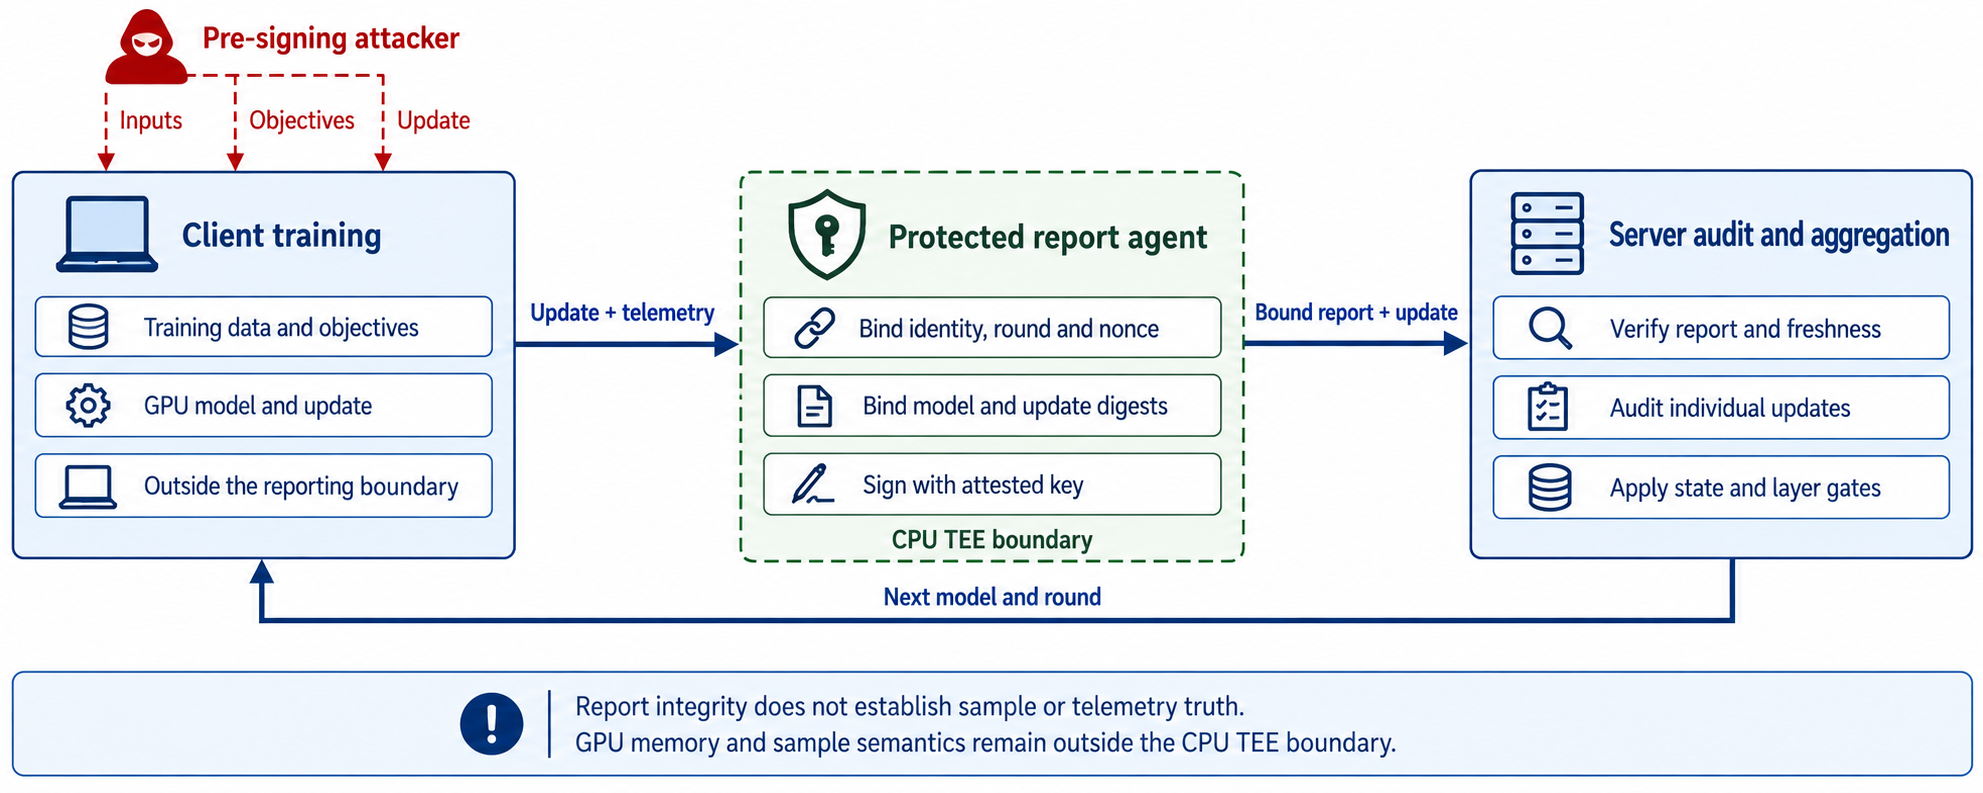
\includegraphics[width=0.94\textwidth]{figures/system_boundary.png}
    \caption{System roles and assumed reporting boundary. Red dashed paths locate
        attacks on inputs, objectives, or updates before signing. The protected
        agent binds identity, freshness, and model/update digests; the server audits
        individual updates before aggregation. The protected process authenticates reports, while content safety remains a
        server-audit responsibility.}
    \label{fig:system_arch}
\end{figure*}

The executable core accepts a valid-admission flag, normalized runtime entropy
$h\in[0,1]$, trainable update blocks, a server reference increment, and measured
proxy loss and activation changes. It does not implement a TEE or a complete
training application. A block is one named, floating-point trainable parameter
tensor in a fixed manifest. Running statistics and integer buffers are excluded
from both this manifest and the controller's output; a training adapter must
handle them separately without treating them as scored learning updates.

\section{Evidence and State Control}
\label{sec:control}

Each round freezes the peer population, audits current updates, advances the
states, and then aggregates eligible parameter blocks, as in
Fig.~\ref{fig:framework}. Let $\mathcal D_t$ contain valid submissions from
clients not previously blacklisted. Before processing any state transition,
freeze
\begin{equation}
    \begin{split}
        \mathcal R_t=\{k\in\mathcal D_t:\; & s_k^{(t-1)}\in
        \{\mathrm{NORMAL},\mathrm{SUSPECT}\},                      \\
                                           & r_k^{(t-1)}<\tau_s\}.
    \end{split}
\end{equation}
A quarantined client supplies recovery evidence but never enters this round's
peer statistics. Here $\tau_s=0.64$ is the review-risk threshold.
Peer comparisons exclude the evaluated client itself.

\begin{figure*}[!t]
    \centering
    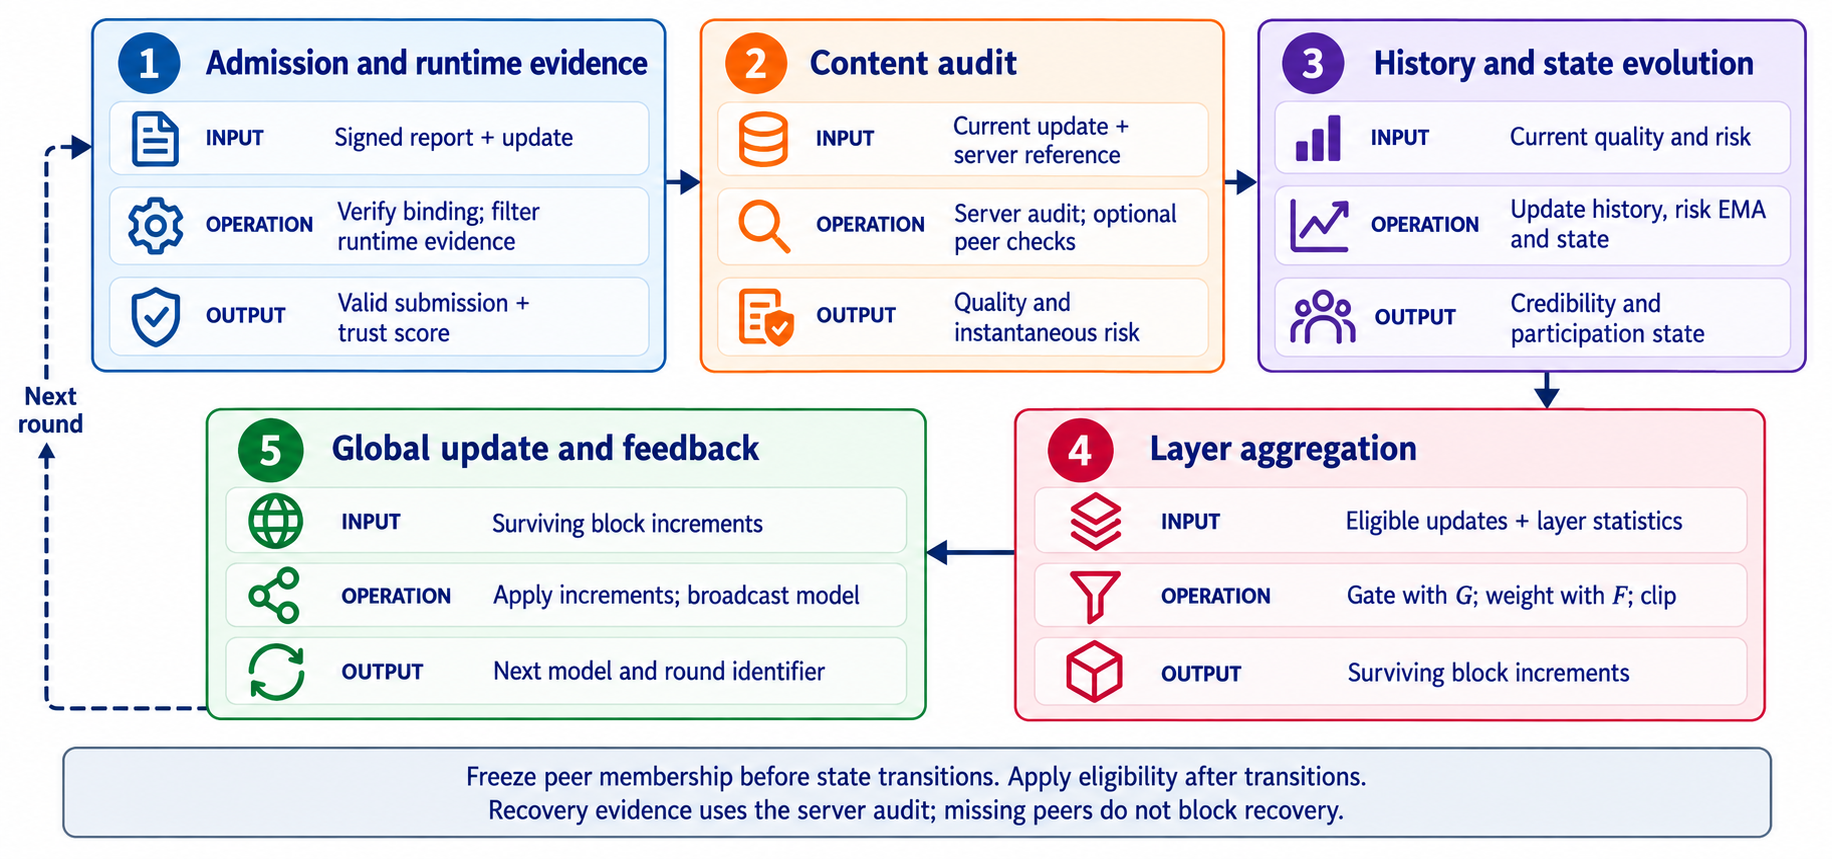
\includegraphics[width=\textwidth]{figures/five_stage_framework.png}
    \caption{Five-stage trust-flow loop. The peer set is frozen before state
        transitions, while aggregation eligibility uses the updated state.
        A client starting in QUARANTINE may provide server-audited recovery
        evidence without entering that round's peer statistics. Recovery to
        SUSPECT restores conditional aggregation eligibility in the same round;
        Section~\ref{sec:transitions} specifies the transition rules.}
    \label{fig:framework}
\end{figure*}

\subsection{Admission and Runtime Reliability}

Let $M_k\in\{0,1\}$ be the admission-verification result. Invalid admission
excludes the update and freezes its temporal state. For valid nonzero
submissions with complete server evidence, the runtime filter uses
\begin{align}
    R_k          & =\exp(\lambda h_k),                 \\
    Z_k          & =w_a+(1-w_a)(1-h_k),                \\
    P_k^-        & =P_k+Q,\quad K_k=P_k^-/(P_k^-+R_k), \\
    T_k'         & =T_k+K_k(Z_k-T_k),                  \\
    P_k'         & =(1-K_k)P_k^-,                      \\
    TrustScore_k & =M_k T_k'/(1+P_k').
\end{align}
The fixed controller parameters are $w_a=0.7$, $\lambda=1$, $Q=0.01$,
$T_0=1$, and $P_0=0.25$. Entropy increases measurement uncertainty and reduces
the observation mean; it is not a label of maliciousness. Tests supply $h$
directly, so their results do not validate a particular telemetry histogram,
instruction-counter collector, or TEE deployment.

\subsection{Server Audit and Optional Peer Evidence}

The mandatory audit uses a server reference and proxy measurements. For a
training adapter, the reference increment is one full-proxy cross-entropy
SGD step, $g=-10^{-3}\nabla_W\mathcal L_{proxy}(W)$, without momentum or weight
decay. The controller consumes the resulting vector. Deterministic tests
supply an explicit reference vector instead of running a model optimizer.

A cosine is available only when both vector norms exceed
$\varepsilon_n=10^{-12}$. An unavailable cosine is omitted from risk fusion;
it is not set to zero and interpreted as disagreement. Let $c_k$ denote the
available reference cosine. The direction risk is $(1-c_k)/2$ and the
reference quality is $v_k=0.6+0.4c_k$. When the reference direction is
unavailable, proxy behavior defines $v_k=(1-r_{loss,k})(1-r_{act,k})$.
For usable peers $j\in\mathcal R_t\setminus\{k\}$, positive trust weights
produce a mean cosine $\bar c_k$ and $S_{\mathrm{peer},k}=0.6+0.4\bar c_k$. Then
\begin{equation}
    q_k=\begin{cases}
        5S_{\mathrm{peer},k}v_k/(4S_{\mathrm{peer},k}+v_k), & \text{usable peers exist}, \\
        v_k,                & \text{otherwise}.
    \end{cases}
\end{equation}
All available quantities lie in $[0,1]$; no peer value is imputed when the set
is empty. The peer-risk channel, when available, is
$r_{peer,k}=\operatorname{clip}(1-\bar c_k,0,1)$.

Write $\Delta\mathcal L_k=\mathcal L_{proxy}(W+\Delta W_k)-
    \mathcal L_{proxy}(W)$. The mandatory server channels are
\begin{align}
    r_{loss,k} & =\operatorname{clip}\left(
    \frac{\max\{0,\Delta\mathcal L_k\}}
    {\delta_{loss}},0,1\right),                                    \\
    r_{act,k}  & =\operatorname{clip}(d_{act,k}/\delta_{act},0,1).
\end{align}
For a batch of $B$ matched inputs and activation vectors $A_i$ at a declared
representation, activation drift is
\begin{equation}
    d_{act,k}=\frac1B\sum_{i=1}^B
    \operatorname{KL}\!\left(\operatorname{softmax}(A_{base,i})
    \Vert\operatorname{softmax}(A_{k,i})\right).
\end{equation}
Softmax is taken over flattened features of each sample, never over the batch.
The same inputs and evaluation mode are used before and after the candidate
update. For a ResNet-18 adapter, the declared representation is the 512-vector
after global average pooling. The array implementation tests this sample axis;
it does not claim a trained ResNet measurement.

Each scale uses trusted calibration observations of its own nonnegative
quantity: $\delta=\max\{10^{-6},\operatorname{median}(z)+3\operatorname{MAD}(z)\}$.
Calibration inputs are separate from final evaluation inputs. Positive scales
are required inputs to the controller. Recovery fixtures use synthetic zero
loss/activation changes and scales of one; those are test inputs, not fitted
CIFAR-10 calibration values.

Amplitude risk is $\operatorname{clip}(\|\Delta W_k\|/m_{\mathrm{norm},k}-1,0,1)$, where
$m_{\mathrm{norm},k}$ is the median nonzero norm of usable peer updates. With no usable peer,
$m_{\mathrm{norm},k}=\|g\|$. The channel is omitted if this scale is at most $\varepsilon_n$.
Instantaneous risk $z_k$ is the maximum of the two mandatory server channels
and all available geometric channels. Missing proxy evidence freezes history,
risk, and counters and yields zero aggregation weight. A full-update norm at
most $\varepsilon_n$ is a no-operation submission with the same freeze rule;
it cannot build reputation or create a direction alarm.

This separates recovery from peer availability: when all clients are
quarantined, valid nonzero updates can still be evaluated against the trusted
server. Loss of the server audit service intentionally suspends recovery;
that external dependency is distinct from a circular peer-state dependency.

\subsection{History, Risk, and Persistent Transitions}
\label{sec:transitions}

Figure~\ref{fig:state_machine} connects the four participation states using
explicit persistence conditions. Historical utility and short-term risk
jointly determine review, while the starting state determines the available
transition. BLACKLIST is enforced by the server rejecting future submissions.

\begin{figure*}[!t]
    \centering
    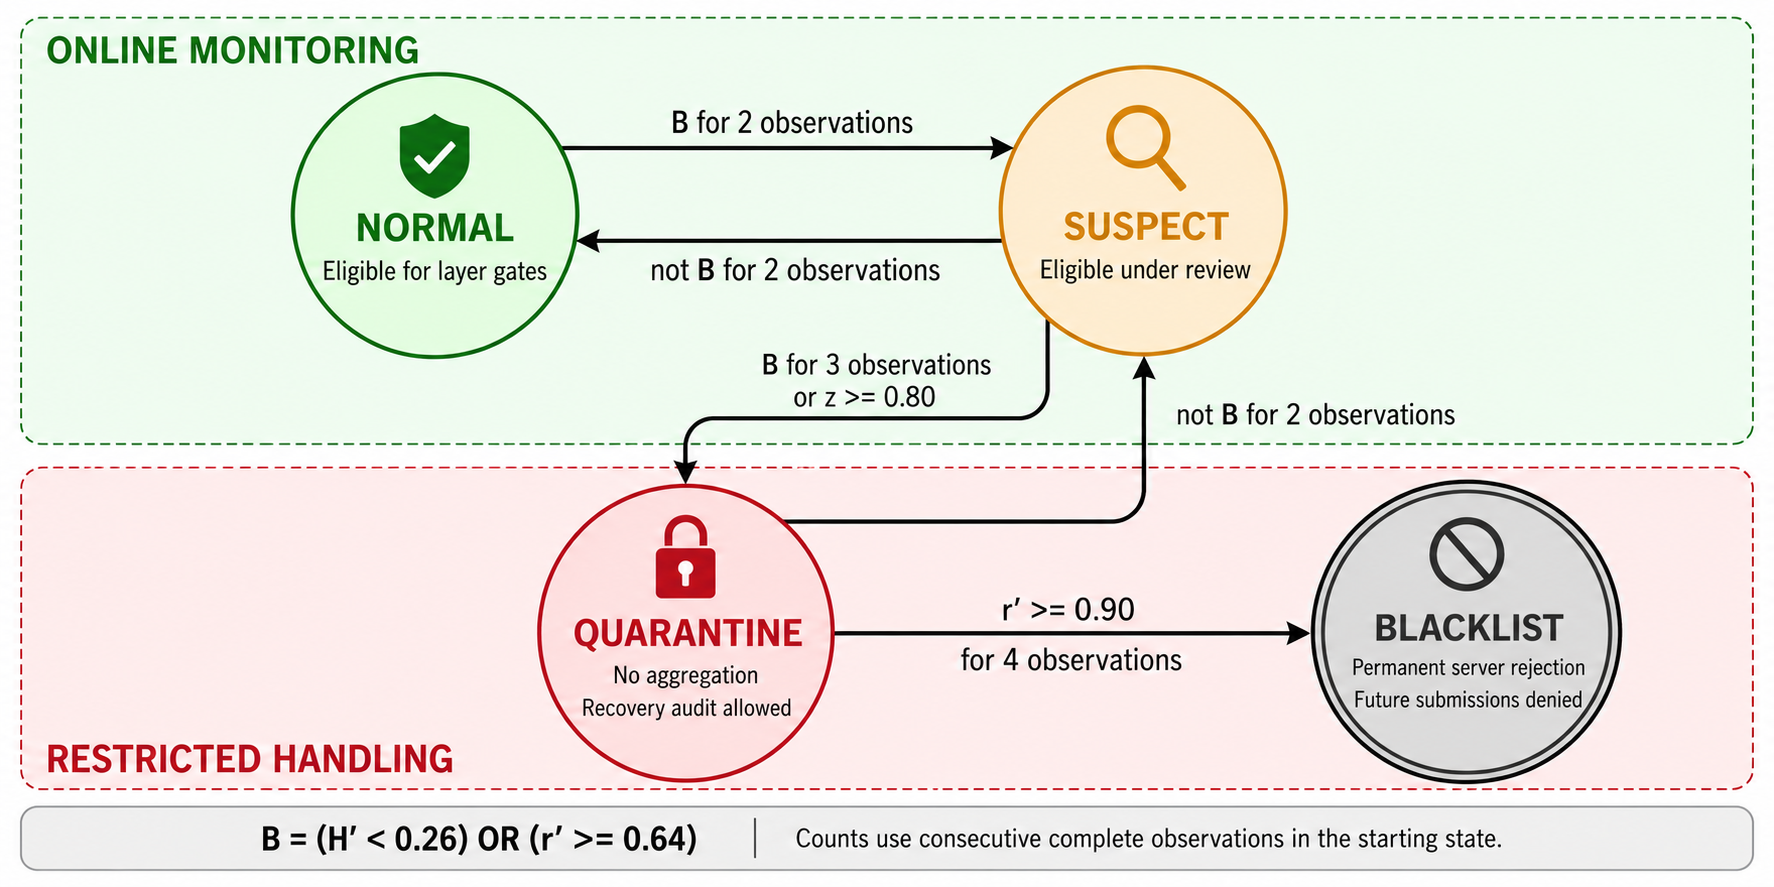
\includegraphics[width=0.90\textwidth]{figures/state_machine.png}
    \caption{Four-state participation policy with explicit transition conditions.
        $B_k=(H_k'<0.26)\lor(r_k'\ge0.64)$; the diagram suppresses the client
        subscript. Counts refer to consecutive complete observations in the
        starting state. Escalation takes priority, and BLACKLIST is terminal.}
    \label{fig:state_machine}
\end{figure*}

Each complete nonzero submission adds unit evidence to the history model:
\begin{align}
    a_k' & =\beta_h a_k+q_k,  & b_k' & =\beta_h b_k+1-q_k,          \\
    H_k' & =a_k'/(a_k'+b_k'), & r_k' & =\beta_r r_k+(1-\beta_r)z_k.
\end{align}
Initialization is $a_0=b_0=1$, $r_0=0$; $\beta_h=0.9$ and $\beta_r=0.85$.
The strictly positive evidence masses require no additive denominator offset.
History and risk share some geometric inputs and are not statistically
independent evidence streams.

\textbf{Utility threshold.} The review condition is
\begin{equation}
    B_k=(H_k'<0.26)\ \lor\ (r_k'\ge0.64).
\end{equation}
Thus 0.26 is a lower bound on historical utility, not a threshold on $1-H_k$.
A favorable recovery observation satisfies $\neg B_k$. Transitions are
evaluated using the starting state and updated
history/risk. At most one transition occurs per complete submission; escalation
has priority. Each counter counts consecutive qualifying observations in its
starting state, resets on a failed condition, and all counters reset after a
transition. Missing or no-operation submissions freeze counters. There is no
instantaneous override of the EMA or extra attack-specific blacklist branch.

From NORMAL, two consecutive $B_k$ observations lead to SUSPECT.
From SUSPECT, three consecutive $B_k$ observations or a current $z_k\ge0.80$
lead to QUARANTINE; two consecutive $\neg B_k$ observations restore NORMAL.
From QUARANTINE, four consecutive $r_k'\ge0.90$ observations lead to BLACKLIST;
otherwise, two consecutive $\neg B_k$ observations restore SUSPECT.

Newly quarantined or blacklisted updates are excluded immediately. BLACKLIST
also rejects future submissions. Recovery to SUSPECT restores conditional
current-round eligibility. Recovery does not itself imply passing a layer gate
or applying a nonzero model update; those endpoints are logged separately.

\section{Aggregation with Attainable Gates}

Figure~\ref{fig:layer_gating} separates the evidence inputs, layer decisions,
and constrained execution. The normalized score $G_k$ determines gate passage,
whereas the raw credibility $F_k$ determines each survivor's relative weight.

\begin{figure*}[!t]
    \centering
    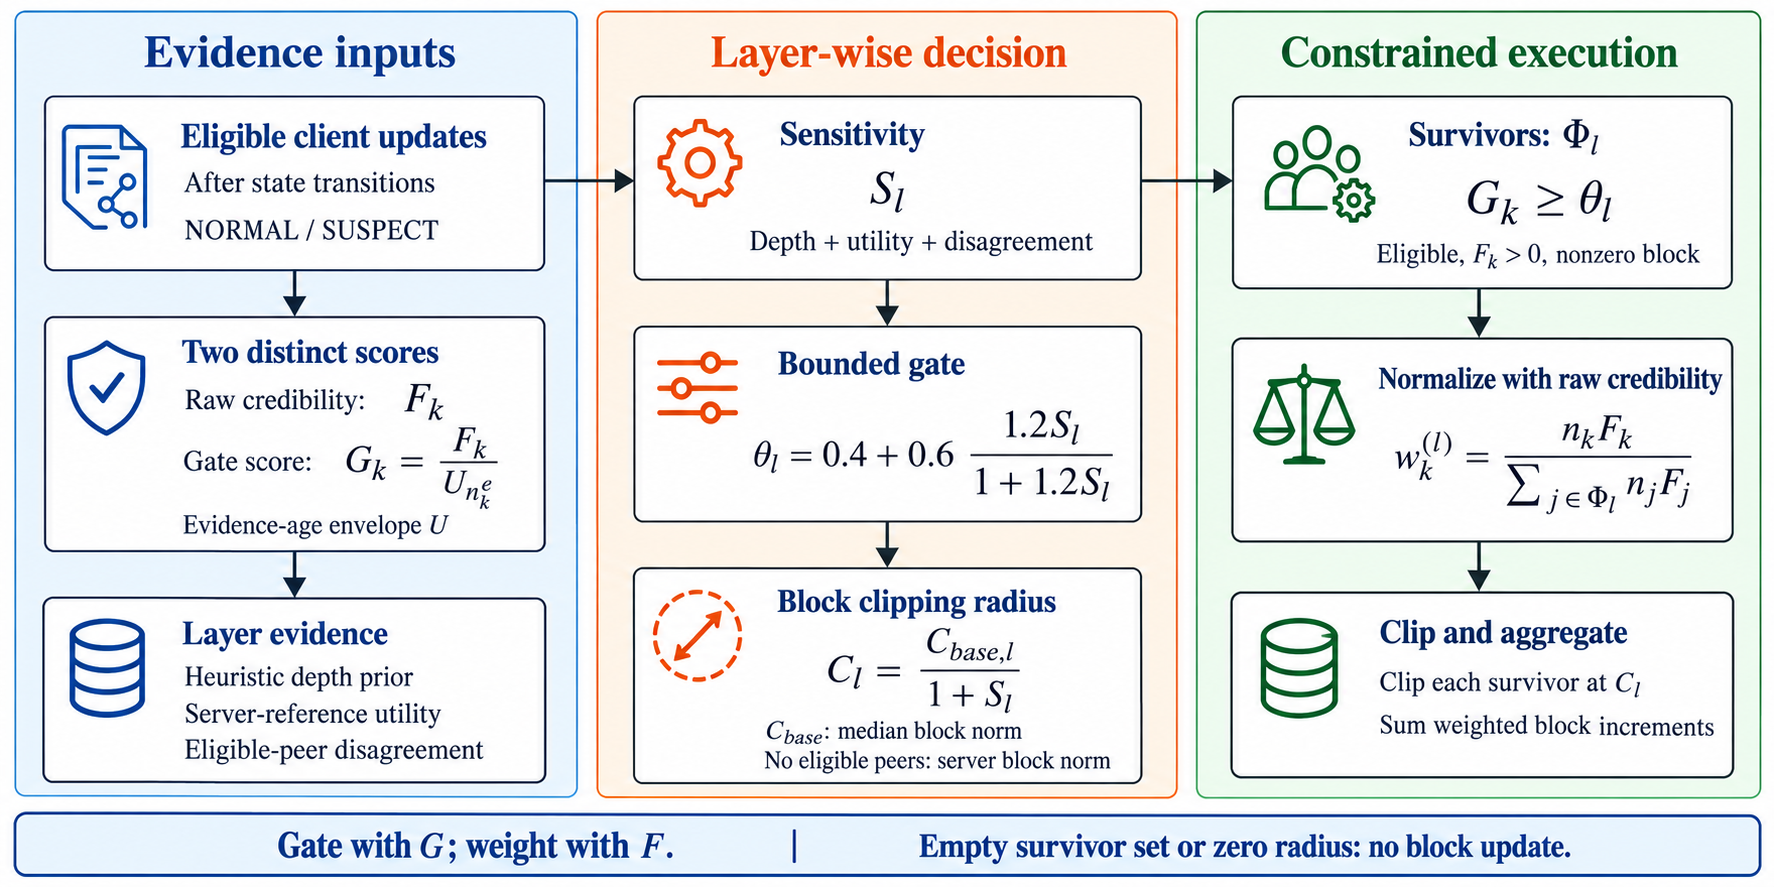
\includegraphics[width=\textwidth]{figures/layer_aggregation.png}
    \caption{Layer-wise aggregation after state transitions. Only eligible
        NORMAL/SUSPECT submissions can survive a gate. The comparison uses
        $G_k=F_k/U_{n_k^e}$, but weights retain $n_kF_k$. Depth is a heuristic
        prior; clipping uses a separate scale for each parameter block.
        An empty survivor set or a radius at most $\varepsilon_n$ produces no
        block update, without bypassing state exclusion.}
    \label{fig:layer_gating}
\end{figure*}

Let $\mathcal E_t$ contain complete nonzero audited submissions. After state
transitions, form $\mathcal A_t=\{k\in\mathcal E_t:
    s_k^{(t)}\in\{\mathrm{NORMAL},\mathrm{SUSPECT}\}\}$.
The unnormalized credibility score remains
\begin{equation}
    F_k=TrustScore_k^3 q_k\sqrt{H_k'}(1-r_k').
\end{equation}
A fixed gate near one is unsuitable because filter uncertainty suppresses the
entire attainable score range. Instead, normalize only the gate comparison by
a deterministic best-evidence envelope at the client's evidence age $n_k^e$.
Here $n_k^e$ counts complete nonzero submissions and is distinct from the
training-record count $n_k$.

Starting from $\underline P_0=0.25$, $a_0^+=b_0^-=1$, define
\begin{align}
    \underline P_n & =\frac{\underline P_{n-1}+Q}{1+\underline P_{n-1}+Q},                          \\
    a_n^+          & =0.9a_{n-1}^++1,                                      & b_n^- & =0.9b_{n-1}^-, \\
    U_n            & =(1+\underline P_n)^{-3}
    \sqrt{a_n^+/(a_n^++b_n^-)}.
\end{align}
Since $R\ge1$, $T\le1$, $q\le1$, and $r\ge0$, induction gives $F_k\le U_{n_k^e}$.
The bound is attained with valid admission, $h=0$, $q=1$, and $z=0$ at every
complete observation. The dimensionless gate score is $G_k=F_k/U_{n_k^e}$;
actual weights continue to use $F_k$, preserving the covariance penalty there.

\subsection{Layer Statistics and Clipping}

Layer statistics use $\mathcal T_t=\mathcal R_t\cap\mathcal A_t$. This is a
current-eligibility filter on the frozen peer set. Newly recovered clients may
aggregate but cannot influence the same-round layer statistics. For blocks
$l=1,\ldots,L$, define
\begin{align}
    S_{depth}^{(l)} & =e^{-3l/L},                                                 \\
    S_{util}^{(l)}  & =\|g^{(l)}\|/\max_m\|g^{(m)}\|,                             \\
    S_{sec}^{(l)}   & =\tfrac12(1-\operatorname{mean}_{k\in\mathcal T_t}
    \cos(\Delta W_k^{(l)},g^{(l)})),                                              \\
    S_l             & =0.3S_{depth}^{(l)}+0.3(1-S_{util}^{(l)})+0.4S_{sec}^{(l)}.
\end{align}
Only available cosines enter the mean. An empty cosine set gives no peer
disagreement contribution, $S_{sec}=0$, and is recorded as missing peer evidence.
If all root blocks have zero norm, set $S_{util}=0$.
The depth component is a heuristic prior, not a measured privacy risk or a
privacy guarantee.

The bounded gate and clipping radius are
\begin{equation}
    \theta_l=0.4+0.6\frac{1.2S_l}{1+1.2S_l},\qquad
    C_l=\frac{C_{base,l}}{1+S_l}.
\end{equation}
Here $C_{base,l}$ is the median norm of block $l$ over $\mathcal T_t$;
it is not the norm of the complete model update. If $\mathcal T_t$ is empty,
use the corresponding server-reference norm $\|g^{(l)}\|$. A radius at most
$\varepsilon_n$ leaves that block unchanged. Thus trusted server evidence also
supplies a defined aggregation path after collective quarantine, without
using quarantined updates to set their own thresholds or clipping radii.

Because $0\le S_l\le1$, $0.4\le\theta_l\le0.727273<1$. The attainable
best-evidence score $G_k=1$ passes every such gate, including at the first
complete submission. This eliminates structural impossibility caused by the
score envelope; it does not guarantee that noisy or heterogeneous updates pass.

\subsection{Survivors and Applied Updates}

For a positive clipping radius, survivors are
\begin{equation}
    \Phi_l=\{k\in\mathcal A_t:G_k\ge\theta_l,\ F_k>0,
    \|\Delta W_k^{(l)}\|>\varepsilon_n\}.
\end{equation}
If $\Phi_l$ is empty, $\Delta W_{global}^{(l)}=0$. No state exclusion or gate
is bypassed by a fallback. Otherwise positive survivor mass permits exact
normalization:
\begin{align}
    w_k^{(l)}                  & =\frac{n_k F_k}{\sum_{j\in\Phi_l}n_j F_j},             \\
    \widehat{\Delta W}_k^{(l)} & =\Delta W_k^{(l)}
    \min\{1,C_l/\|\Delta W_k^{(l)}\|\},                                                 \\
    \Delta W_{global}^{(l)}    & =\sum_{k\in\Phi_l}w_k^{(l)}\widehat{\Delta W}_k^{(l)}.
\end{align}
Weights sum to one on a nonempty survivor set. Each clipped block norm is at
most $C_l$, so the triangle inequality also bounds the aggregate norm by $C_l$.
Individual nonzero contributions can cancel; a selected block, a positive
weight, and a nonzero aggregate increment are therefore distinct endpoints.

The audit records client, round, trainable-block name, starting/ending state,
quality, instantaneous and smoothed risk, history, persistence counters,
transition reason, raw and gate scores, threshold, survivor membership,
normalized weight, pre/post-clipping norms, and applied contribution norm.
Per-block logs additionally record survivor count, clipping radius, skipped
updates, and the norm of the summed increment.

\section{Training Study}
\label{sec:original_study}

\subsection{Protocol, Provenance, and Metrics}

The CIFAR-10 results in this section concern the original training
implementation. The author-confirmed protocol uses five matched seed, partition,
and attack schedules on each of Intel and AMD platforms, giving ten
platform--seed runs. Table~\ref{tab:training_setup} records this study's settings;
it does not infer training settings from the controller fixtures. Admission
tests additionally used five Sybil and three free-rider identities that were
rejected before the twenty-client training statistics were collected.
The supplied figures are confirmed by the authors as measurements, but their
individual platform/seed identifiers and the complete aggregation script are
not available in the current reproducibility bundle. The study summary and
representative curves therefore have distinct statistical roles. The model and
partition manifest associated with each retained curve is also not independently
linked to Table~\ref{tab:training_setup}; the curves provide descriptive
training evidence rather than a newly matched comparison.
Section~\ref{sec:verification} separately checks the explicit controller;
no unchanged training behavior is inferred for its recovery, gate, or clipping
refinements.

\begin{table}[!htb]
    \centering
    \caption{Reported training protocol. Missing run-level details are stated
        explicitly; controller-test parameters do not fill those gaps.}
    \label{tab:training_setup}
    \small
    \setlength{\tabcolsep}{3pt}
    \begin{tabular}{@{}p{1.65cm}p{6.2cm}@{}}
        \toprule
        Item & Training-study setting \\
        \midrule
        Model & CIFAR-10 ResNet-18: $3\!\times\!3$ stride-1 stem, no initial
        max pool, ten outputs; initialization checkpoint/seed list unavailable. \\
        Clients & 20 admitted clients; 14 benign and 6 malicious. \\
        Partition & 45,000 exclusive training images: clients 0--9 IID,
        10--14 Dirichlet $\alpha=1$, 15--19 $\alpha=0.1$. \\
        Shared pool & 5,000 training images copied to every client, in addition
        to its exclusive partition; each local copy counts in $n_k$. \\
        Server proxy & 500 balanced CIFAR-10 test-source images (50/class),
        excluded from client training; exact indices unavailable. \\
        Attacks & C0 label flipping ($0.5$); C1 trigger, C2 clean-label,
        C3 semantic; C4 sign flipping; C5 $100\times$ scaling. \\
        Optimizer & SGD, learning rate $0.001$, momentum $0.9$; three local
        epochs; 30 rounds for the main study, 50 for aggregation comparison. \\
        Repetitions & Intel and AMD, five matched schedules each; ten-run
        reported mean and SD, without a platform-effect test. \\
        Evaluation & Clean accuracy and reported targeted ASR; final-test and
        calibration indices, overlap audit, and per-attack counts unavailable. \\
        \bottomrule
    \end{tabular}
\end{table}

The trigger attack modifies 20\% of local samples with a bottom-right
$3\times3$ patch and target class 0. The clean-label and semantic attacks also
use 20\% subsets and target class 0; their perturbation budget and semantic
attribute are not recoverable from the supplied study description. The five
matched schedules control repeated data/attack randomization across platforms;
ten platform--seed observations do not imply ten independent partitions.
The shared pool is 10\% of unique training images, not 10\% of each client's
local dataset. Its local fraction is $5000/(5000+n_k^{\mathrm{exclusive}})$.
The Dirichlet parameters describe the exclusive portions; a shared component
remains present in every client.

Clean accuracy is the fraction of correctly classified evaluation images.
For targeted attack $a$, the reported definition is
$\mathrm{ASR}_a=|\{x\in\mathcal B_a:\arg\max f(x)=y_a^*\}|/|\mathcal B_a|$,
and the study reports the macro-average over trigger, clean-label, and semantic
attacks. The underlying per-attack counts and target-class exclusion rule are
not supplied, so these values cannot be recomputed under a harmonized ASR
protocol. Untargeted label/sign/scaling attacks are not terms in that average.
Permanent-ban FPR counts benign clients ending in BLACKLIST, not temporary
review or quarantine. Because the proxy originates from the test-source split,
independence from final evaluation requires an index-level check that is not
available here; held-out generalization is not established by this provenance.

\subsection{Main Performance and Client Behavior}

Table~\ref{tab:training_summary} retains the author-confirmed TTFL summary
from the original manuscript. It is a reported aggregate, not a recomputation
from partial local logs. Baseline rows without a complete matching run record
are omitted from this table, so it supports no new method-ranking or
significance claim. The zero permanent-ban FPR describes the tested benign
clients; it does not imply that all their updates passed every layer gate.

\begin{table}[!htb]
    \centering
    \caption{Reported TTFL training summary under 30\% mixed attacks.
        Accuracy and ASR are the reported mean $\pm$ SD over ten platform--seed
        runs; the per-attack ASR audit remains incomplete.}
    \label{tab:training_summary}
    \small
    \begin{tabular}{@{}lc@{}}
        \toprule
        Metric & Reported value (\%) \\
        \midrule
        Clean accuracy & $92.31\pm0.09$ \\
        Targeted ASR (reported macro-average) & $10.21\pm0.05$ \\
        Benign permanent-ban FPR & $0.00$ \\
        \bottomrule
    \end{tabular}
\end{table}

Figure~\ref{fig:main_results}(a) shows the measured accuracy and recorded
backdoor-ASR trajectories. The red series is an attack-success measurement,
not a fixed reference line. Its mapping to the three per-attack outcomes is
not documented, so it is not identified with the macro-average at every round.
The displayed accuracy endpoint is 92.30\%, whereas Table~\ref{tab:training_summary}
reports the repeated-run mean of 92.31\%; the curve is not used to recover that
mean or its SD. Figure~\ref{fig:main_results}(b) shows distinct historical-utility
and risk trajectories. Its detection, interception, and isolation annotations
retain their original meanings and are not converted into BLACKLIST times for
the executable controller. Together the panels describe learning and client
behavior without equating temporary restriction with permanent removal.

\begin{figure*}[!t]
    \centering
    \begin{minipage}[t]{0.49\textwidth}
        \vspace{0pt}
        \centering
        {\small\bfseries Training accuracy and recorded backdoor ASR\par}
        \smallskip
        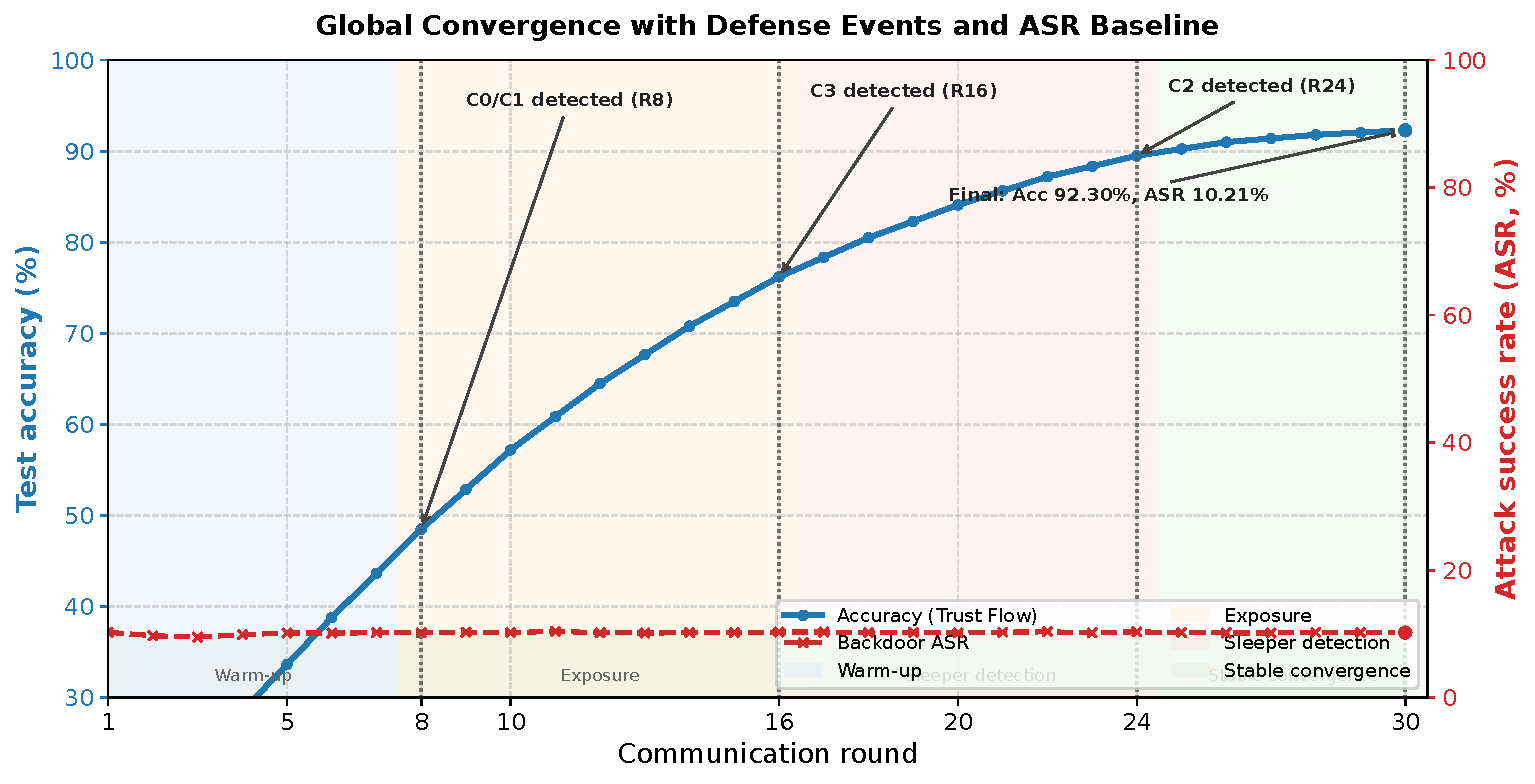
\includegraphics[width=\linewidth,trim=0 0 0 21bp,clip]{figures/fig6_convergence_asr.pdf}
        \par\smallskip
        {\footnotesize (a) Accuracy and measured attack-success trajectory.}
    \end{minipage}\hfill
    \begin{minipage}[t]{0.49\textwidth}
        \vspace{0pt}
        \centering
        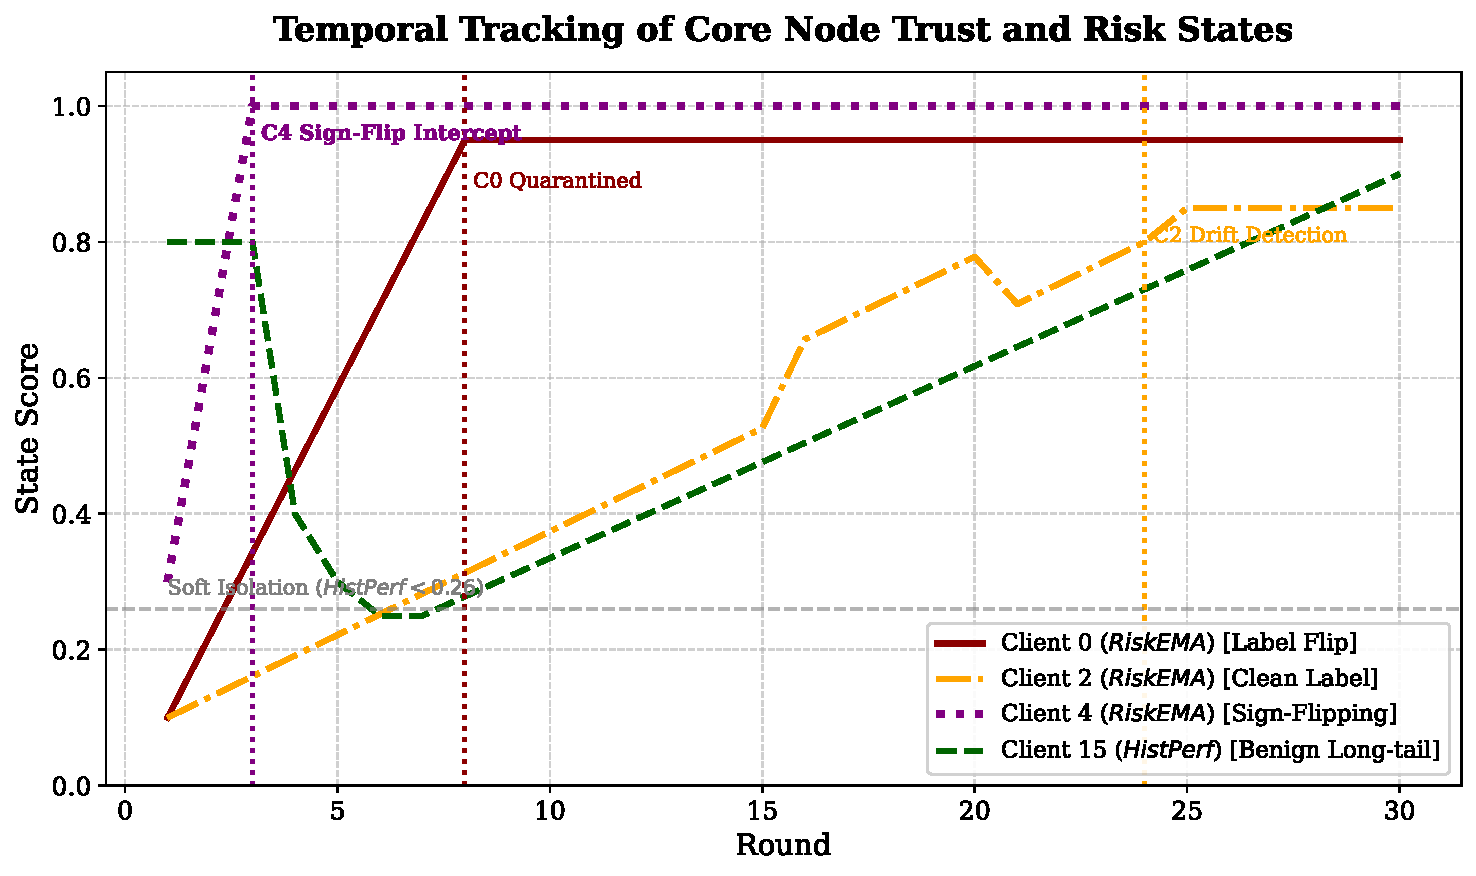
\includegraphics[width=\linewidth]{figures/fig7_node_state_evolution_ispa.pdf}
        \par\smallskip
        {\footnotesize (b) Client historical utility and risk.}
    \end{minipage}
    \caption{CIFAR-10 training behavior: (a) accuracy and recorded backdoor ASR
        over 30 rounds; (b) representative client trajectories with detection
        and restriction events. Curves describe the training implementation,
        not the constructed controller tests.}
    \label{fig:main_results}
\end{figure*}

\subsection{Aggregation Variants and Data Partitions}

Figure~\ref{fig:aggregation_partitions}(a) compares three operations over
50 rounds. Global-Clipping applies a common clipping policy; hierarchical
gating without renormalization removes disallowed layer contributions without
redistributing their weights; the full method normalizes weights over each
layer's survivors. The displayed curves also differ in gating and clipping,
so the full performance gap cannot be attributed solely to normalization.
The 30-round marker is a within-curve reference, not the end of this comparison.

Figure~\ref{fig:aggregation_partitions}(b) compares the reported Dirichlet
settings. The TTFL series changes less across the displayed settings than
Krum and FLTrust. The shared pool remains part of the training protocol;
$\alpha$ describes the exclusive data rather than the full local distribution.
The sweep's exact per-client allocation manifests and repeated-run summaries
are unavailable, so the plot does not establish distribution-independent
robustness or isolate the effect of the shared pool.

\begin{figure*}[!t]
    \centering
    \begin{minipage}[t]{0.49\textwidth}
        \vspace{0pt}
        \centering
        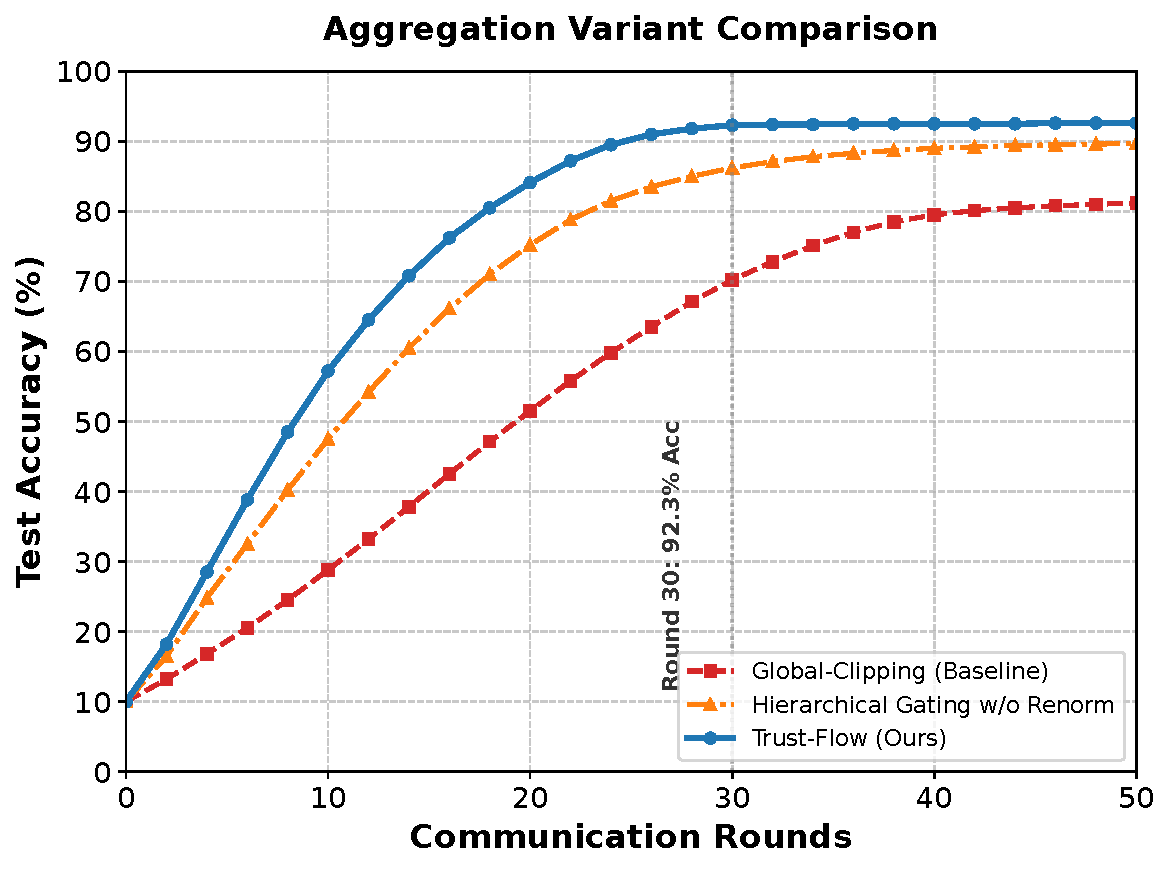
\includegraphics[width=\linewidth]{figures/fig10_ablation_renorm.pdf}
        \par\smallskip
        {\footnotesize (a) Aggregation variants over 50 rounds.}
    \end{minipage}\hfill
    \begin{minipage}[t]{0.49\textwidth}
        \vspace{0pt}
        \centering
        % Cover only the old title band; all axes and data stay visible.
        \begingroup
        \setlength{\unitlength}{\linewidth}
        \begin{picture}(1,0.65866)
            \put(0,0){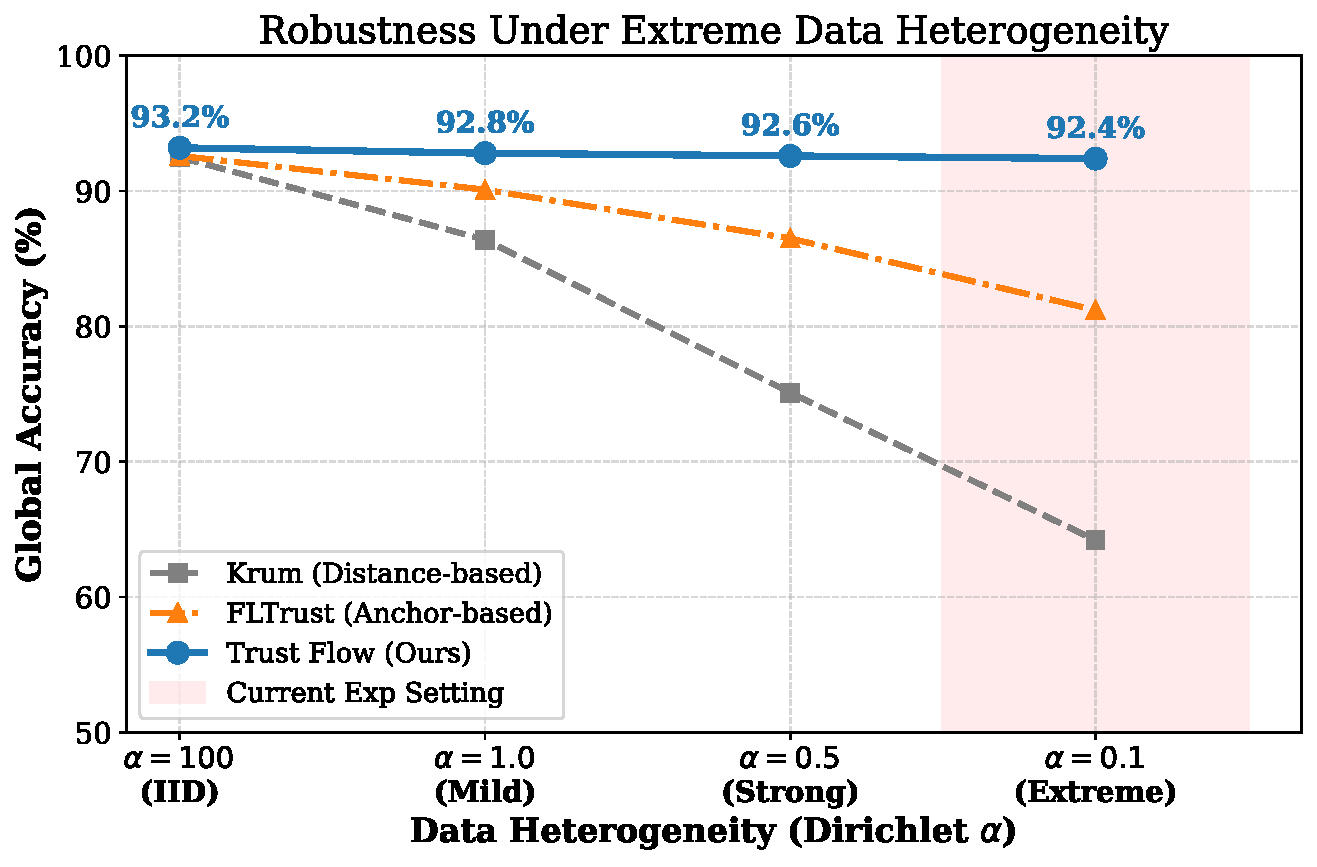
\includegraphics[width=\linewidth]{figures/fig11_alpha_sensitivity_ispa.pdf}}
            \put(0.13,0.618){\color{white}\rule{0.87\linewidth}{0.041\linewidth}}
            \put(0.56,0.635){\makebox(0,0){\small\bfseries Accuracy across data-partition settings}}
        \end{picture}
        \endgroup
        \par\smallskip
        {\footnotesize (b) Accuracy at the reported Dirichlet settings.}
    \end{minipage}
    \caption{Training-study comparisons. (a) Global clipping, hierarchical
        gating without weight renormalization, and full TTFL; the comparison
        changes multiple aggregation operations. (b) Accuracy across exclusive-data
        partition settings in the presence of a shared training pool. No
        unreported uncertainty estimates are inferred from either panel.}
    \label{fig:aggregation_partitions}
\end{figure*}

\FloatBarrier
\section{Executable Protocol Verification}
\label{sec:verification}

\subsection{Scope and Reproduction}

The controller in \path{protocol/controller.py} implements the
specified audit, temporal states, and aggregation; \texttt{config.json} fixes
its parameters. Eleven test groups export state, block, and layer events with
source hashes. These are constructed control tests, not classifier training.
The randomized check uses seed 20261001 and 100 sequences of 100 observations.
Table~\ref{tab:verification} in the appendix lists the conditions and endpoints.

The partial training-code snapshot differs in its history update, raw-score
gating, clipping scales, and weighting. It is not the complete implementation
underlying Section~\ref{sec:original_study}, so a matched training comparison
is still needed to quantify the effect of the explicit controller rules.

\subsection{Recovery and Startup Behavior}

A counterexample combines the deliberately incorrect cutoff $H<0.74$ with
mandatory peers: $q=0.8$, $z=0.3$ lead to quarantine at observation five and
frozen history through forty. This does not describe the training
implementation, whose state annotation already uses $H<0.26$. With that
utility floor, the constructed startup sequence remains NORMAL.

The matched recovery test instead initializes twenty clients in QUARANTINE
with risk 0.95, history 0.5, and reset counters. Each submits the server-aligned
update $(1,0)$ with zero loss/activation change, unit calibration scales, and
zero entropy. Thus $q=1$, $z=0$ despite an empty peer set. Risk falls below
0.64 at audit three; the next favorable observation restores SUSPECT and
nonzero aggregation at four. All clients return to NORMAL at six
(Fig.~\ref{fig:recovery}). In the matched arm, only the requirement for usable
peers before state advancement changes. All clients remain quarantined and
aggregation remains zero through ten attempted audits. This isolates the peer
dependency under favorable server evidence; it is not a training comparison or
a universal guarantee of benign recovery.

\subsection{Risk Timing and Gate Reachability}

With $r_0=0$ and $z_t\le1$, pure EMA satisfies $r_t\le1-0.85^t$.
At $t=14$ its upper bound is $0.89723$, below the blacklist threshold; the
first crossing is at $t=15$. Four consecutive qualifying observations while
quarantined therefore cannot finish before $t=18$. The maximal-risk test
matches that bound and rejects the next submission at $t=19$.

An unscaled gate $0.4+1.2S_l$ can exceed the first-observation raw-score
ceiling $0.469222$, or the asymptotic ceiling of about $0.761393$. The normalized
comparison instead attains one under ideal evidence at every age, while its
maximum gate is $0.727273$. The 10,100 age--sensitivity checks verify these
formulas. They establish gate reachability, not an acceptable survivor rate
on trained models.

\FloatBarrier
\section{Limitations and Conclusion}

TTFL combines authenticated reports, current-update audits, separate utility
and risk streams, and layer-wise aggregation. The training study characterizes
model and client behavior under mixed attacks; the controller checks establish
conditional recovery, attainable gates, and bounded normalized aggregation.
The matched constructed test shows why recovery audits must remain available
when eligible peers disappear.

The training summary does not measure the effect of these controller
refinements. That requires matched training, run-level configuration identities,
per-attack counts, and disjoint proxy/calibration/evaluation indices. The shared
pool also limits the heterogeneity analysis. The partial code cannot establish
full implementation correspondence. Hardware attestation performance, general
Byzantine robustness, and superiority over a tuned single-stream policy remain
outside the verified claims.

\FloatBarrier
\appendices
\section{Supplementary Controller Checks}

\begin{table}[!htb]
    \centering
    \caption{Constructed controller checks and verified endpoints.}
    \label{tab:verification}
    \footnotesize
    \setlength{\tabcolsep}{3pt}
    \begin{tabular}{@{}p{1.75cm}p{6.2cm}@{}}
        \toprule
        Case & Condition and checked endpoint \\
        \midrule
        Cutoff/peers & $q=0.8$, $z=0.3$, cutoff $0.74$,
        mandatory peers: SUSPECT at 2, QUARANTINE at 5; frozen through 40. \\
        Healthy startup & Same $q,z$, utility floor $0.26$: NORMAL through 40
        complete observations. \\
        Collective recovery & 20 quarantined clients, $r_0=0.95$: server audit
        restores aggregation at 4, NORMAL at 6; matched mandatory-peer arm
        stays frozen with zero aggregate through 10. \\
        Maximal risk & $q=z=1$, $r_0=0$: SUSPECT at 8, QUARANTINE at 9,
        BLACKLIST at 18. \\
        Gate envelope & Ideal evidence at 100 ages and 101 sensitivities:
        all 10,100 gate checks pass. \\
        Empty survivors & Low-score candidate plus high-score quarantined
        client: zero increment, no backfill. \\
        Missing evidence & Missing proxy freezes state; server audit with
        one client gives sole-survivor weight 1. \\
        Zero/tiny updates & Norms $0$, $10^{-15}$, $10^{-12}$: no direction
        alarm, history gain, or applied update. \\
        Weights/ clipping & Equal scores, sample counts $1:3$: weights
        $0.25/0.75$; aggregate norm bounded by the radius. \\
        Calibration & Zero calibration inputs: positive
        $10^{-6}$ floor; two-sample KL uses feature-wise softmax. \\
        Random inputs & 100 sequences of 100 observations:
        bounded states/scores; excluded states have no eligibility. \\
        \bottomrule
    \end{tabular}
\end{table}

\subsection{Constructed Recovery Trace}

Figure~\ref{fig:recovery} shows the fixed-input controller test described in
Section~\ref{sec:verification}. All clients submit the same two-dimensional
update at every audit. The discrete state steps and constant applied-update
norm after recovery follow from those test inputs; they are not classifier
learning curves.

\begin{figure}[!htb]
    \centering
    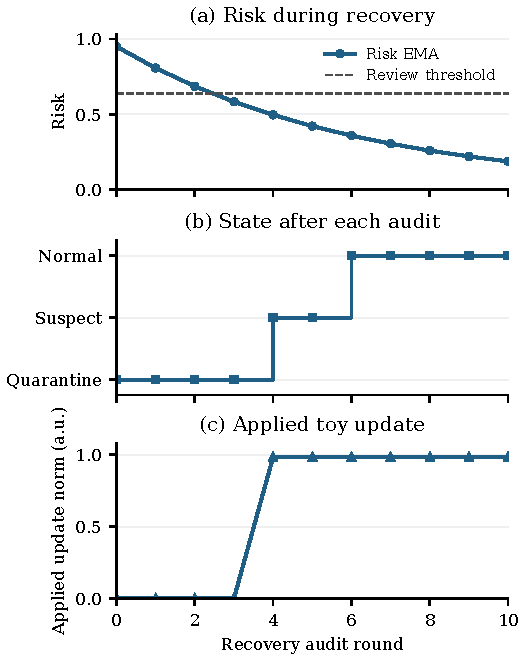
\includegraphics[width=\columnwidth]{figures/collective_recovery.pdf}
    \caption{Constructed collective recovery: common risk/state trajectory
        for twenty clients and applied two-dimensional update norm in arbitrary
        units.}
    \label{fig:recovery}
\end{figure}

\clearpage
\IEEEtriggeratref{11}
\bibliographystyle{IEEEtran}
\bibliography{ispa2026_references}
\end{document}
